\documentclass[11pt]{amsart}
\usepackage[margin=1in]{geometry}
\usepackage{amsmath,amssymb,amsthm,mathtools}
\usepackage{booktabs,enumitem,array,graphicx,xcolor}
\usepackage{tikz}
\usetikzlibrary{positioning,arrows.meta}
\usepackage[colorlinks=true,linkcolor=blue!50!black,citecolor=green!35!black,urlcolor=blue!50!black]{hyperref}

\newtheorem{theorem}{Theorem}[section]
\newtheorem{proposition}[theorem]{Proposition}
\newtheorem{lemma}[theorem]{Lemma}
\newtheorem*{maintheorem}{Main Theorem}
\theoremstyle{definition}
\newtheorem{definition}[theorem]{Definition}
\newtheorem*{hypF}{Former Hypothesis (F) (far-field window estimates; superseded, no longer assumed)}
\newtheorem*{hypO}{Former Hypothesis (O) (outer cutoff of Lemma~S(A); superseded, no longer assumed)}
\theoremstyle{remark}
\newtheorem{remark}[theorem]{Remark}

\newcommand{\R}{\mathbb{R}}
\newcommand{\eps}{\varepsilon}
\newcommand{\ip}[2]{\langle #1,#2\rangle}
\newcommand{\Lam}{\Lambda}
\newcommand{\norm}[1]{\lVert #1\rVert}
\newcommand{\fn}[1]{\texttt{\detokenize{#1}}}
\newcommand{\dref}[1]{[\textsf{#1}]}
\newcommand{\Sset}{\mathcal S}
\newcommand{\pth}[1]{\nolinkurl{#1}}
\raggedbottom
\setlength{\emergencystretch}{2em}

% ======================================================================
% GAP STATEMENT.  The body of this macro is typeset as former Hypothesis (F) in
% Section 1.3 (historical remark); in v3.3 the Main Theorem is NOT conditional on it.  Draft wording
% (from Lemma S(B), Proposition B' of step 3 v3.2 and the gap note
% step3_gap_v32/gap_v32.tex); the authors may replace it.
% ======================================================================
\newcommand{\GAPSTATEMENT}{%
Let $\gamma$ satisfy the hand-off conditions \textup{(H1)--(H6)} of step~3 \textup{v3.2} at $t_1$ \textup{(Theorem~\ref{thm:W})}, and let $\tau'\ge\tau_1$ be such that the bootstrap hypotheses \textup{B1--B4} of step~3 \textup{(\S\ref{ss:boot})} hold on $[\tau_1,\tau']$.

\emph{Windows.} For a window $W=[r_E,\frac32r_E]$ fixed in physical space and present from its entry time $\tau_e$ \textup{(}$\tau_e=\tau_1$ for the windows present at $\tau_1$, among them those covering the strip $r\in[50,150)\lambda_1$; otherwise the time at which $W$ enters through $y=48$\textup{)}, let $\hat E^W_j(\tau)$ be the level-$j$ energy of Proposition~B$'$ of step~3 \textup{(}deviation $v=f-U_e$ from the slow-manifold profile $U_e$ frozen at entry, $z_j=(y\partial_y)^jv$, weight $\hat\omega=28\lambda(\tau_e)/r$ frozen at entry\textup{)}, localised by a cutoff that equals $1$ on $W$ and is supported on $W$ and two edge ramps fixed in physical space. Thus $\hat E^W_j$ bounds the energy on $W$, and in its evolution the total derivatives that the energy identities of Lemma~S discard appear as the fourth-order edge \textup{(}ramp\textup{)} terms.

\emph{Shells.} Let $E^{(A)}_j$ be the shell energies of Lemma~S\textup{(A)}, cut off at an outer ramp in $y>60$ whose fourth-order terms are kept, with their coefficients beyond the core \textup{(}$y>60$\textup{)} bounded by the window box of \textup{(F1)}.

Then for all $\tau\in[\tau_1,\tau']$:
\begin{enumerate}[label=\textup{(F\arabic*)},leftmargin=2.6em,itemsep=1pt]
\item $\hat E^W_j(\tau)<2\,\hat E^W_j(\tau_e)$ for every window and every level used in step~3 \textup{(}levels $0$--$3$ on the windows present at $\tau_1$, levels $0$--$2$ on the windows entering later\textup{)}; and on the window region $y\in[48,R(\tau)]$ the curve is a graph over the $S_1$ ray with $|f|<\frac12$, the per-window boxes of step~3 \textup{\S3.7} hold strictly, and the curvature is at most $S^f_1/r$ \textup{(}notation of step~3\textup{)}. This is \textup{B3} with strict inequalities; it gives the window part of \textup{W4}.
\item $E^{(A)}_j(\tau)<2\hat E_j$, $j=0,1,2$, with $\hat E=(3.12\cdot10^{-7},\,1.81\cdot10^{-4},\,0.248)$, and the core bounds $\sup|v|<0.0153$, $M_0<0.11$, $M_1<0.52$ of \textup{B2} hold on $y\in[28,60]$.
\end{enumerate}
In words: the steps \textup{D3} and \textup{D4} of the bootstrap of step~3 hold, with the bootstrap bounds stated there, once the fourth-order terms at the window edges and at the outer end of the shells are kept.}

\title[CDF singularity from an embedded hair clip]{A curve diffusion singularity from an embedded hair clip, modelled on a non-embedded shrinker}
\author{Micah Warren}
\address{University of Oregon}
\author{Jacob Ogden}
\date{Main-theorem document of a computer-assisted proof. Draft v3 of November 13, 2026 (v3.3 of step 3)}

\begin{document}
\begin{abstract}
Curve diffusion flow (CDF) moves a plane curve with normal velocity $-\kappa_{ss}$. We give an explicit closed curve $\Gamma_0$, a symmetric ``hair clip'' whose tangent angle is an exact sine series with $3762$ terms, certify that it is embedded, and prove, subject to the pending independent review and compilation recorded in the status box below, that its CDF evolution develops a curvature singularity in finite time at a single point, at the self-similar rate, with rescaled profile trapped near the one-loop shrinker $S_1$. Since $S_1$ has a transverse double point, the flow must lose embeddedness before the singular time; in floating-point runs it does so at $t\approx0.003$. The proof has four computer-assisted steps: existence of $S_1$ with tight enclosures; linear stability of $S_1$ modulo symmetries; nonlinear trapping near $S_1$ in rescaled variables; and validated integration from $\Gamma_0$ to a hand-off time $t_1$. Every certified quantity is computed in interval or ball arithmetic with outward rounding. This document states the result, summarises the four steps and their certificates, and records exactly what is open.
\end{abstract}
\maketitle

\begin{center}\fbox{\parbox{0.95\linewidth}{\small\textbf{Status (13 November 2026).} Steps 1, 2, 3 (v3.3) and 4 are complete as written; the items the step documents still list are collected in \S\ref{s:open}. \textbf{The Main Theorem is stated unconditionally, subject to the pending independent review (task 8 of the v3.3 plan) and compilation of the new step-3 text; see \fn{V33_INDEX.md}. A re-review (14 November, \fn{t8_review/REREVIEW_v33.md}) found no blocking item; its findings N1 (chart identification, now closed by the step-4 stage \fn{n1\_chart}) and N2--N5 are handled in \fn{fix2/N35_REPORT.md}. What the theorem still depends on, besides the review and compilation: the literature statements (P1$'$) (the $L^2$ blow-up criterion, Dziuk--Kuwert--Sch\"atzle Theorem~3.1 and/or Chou; \textbf{[to be confirmed by the authors]}) and (P3$'$).} Earlier drafts of this document were conditional on Hypotheses (F1) and (O) (\S\ref{ss:gap}). In v3.3 the far-field estimate is Lemma~U, a uniformly local energy estimate with certified margins, and the outer cutoff of Lemma~S(A) on $[350,700]$ is treated in the repaired Lemma~S(A) rather than assumed; the hand-off gains the item (H2f), a datum on $[60,700]$, and a tightened (H2), both certified in new step-4 stages (\S\ref{s:step4}). The LaTeX of the new step-3 text (\fn{lemmaU.tex}) has not been compiled, its numbers are quoted from certified JSON outputs of new scripts that no second reader has yet seen, and the v3.1 erratum is in \fn{erratum/erratum.tex}. Reproduction on a second machine (Windows~11, Intel i7-10700): step-3 kit (as of v3.1) and step-4 kit~A done; kit~B and the v3.3 kits are pending (\S\ref{ss:repro}).}}\end{center}

\section{Introduction}\label{s:intro}

\subsection{Curve diffusion flow}
Let $\gamma(\cdot,t)$ be closed immersed plane curves with arclength $s$, unit tangent $T=\gamma_s=e^{i\theta}$, normal $\nu=iT$ and curvature $\kappa=\theta_s$. Curve diffusion flow is
\begin{equation}\label{eq:cdf}
\partial_t\gamma=-\kappa_{ss}\,\nu\qquad(\text{modulo tangential terms}).
\end{equation}
It is the one-dimensional case of Mullins' surface diffusion \cite{Mullins1957} and the steepest descent $H^{-1}$-gradient flow of length \cite{Wheeler2013}; it preserves the signed enclosed area $A$ and decreases the length, $\frac{d}{dt}L=-\int\kappa_s^2\,ds$. Local existence for closed curves and global existence near circles are due to Elliott and Garcke \cite{ElliottGarcke1997}; existence and uniqueness for immersed hypersurfaces, and convergence near spheres, to Escher, Mayer and Simonett \cite{EscherMayerSimonett1998}; for closed curves near circles Wheeler proved global existence, exponential convergence and eventual convexity \cite{Wheeler2013}.

\subsection{Why singularities of fourth-order flows are subtle}
For curve-shortening flow (normal velocity $\kappa$), the maximum principle keeps embedded curves embedded, and they shrink to round points \cite{Grayson1987}. CDF has no maximum or comparison principle. Embedded curves can lose embeddedness and convex curves can lose convexity \cite{GigaIto1998,GigaIto1999,MayerSimonett2000,Blatt2010}. This changes the singularity problem in two ways.
\begin{itemize}[leftmargin=*,itemsep=1pt]
\item \emph{No soft criterion applies to embedded data.} An embedded closed curve has turning number $\omega=\pm1$ and $\omega A>0$, both conserved, and the round circle of area $A$ is always an admissible limit; so criteria in terms of these quantities cannot force a singularity, which must come from the dynamics (working notes of Ogden and Warren \dref{OW}, \S2). Known results on finite-time singularities of CDF concern immersed curves, for instance curves of turning number zero or multiply wound curves \cite{Chou2003,EscherIto2005,EGMWW2015}; see \dref{OW} \S2.
\item \emph{The singularity model need not be embedded,} even when the initial curve is: the flow can pass through self-intersections first. Ours does. Its model, the shrinker $S_1$, has a transverse double point.
\end{itemize}
The scenario is that of \dref{OW}: in a long clip with a narrow slot that ends in a small chamber, the chamber becomes a loop, the neck becomes a transverse double point, and the loop collapses self-similarly with profile $S_1$. The slot and chamber are ``$S_1$ with its crossing resolved'' (Figure~\ref{fig:curves}).

\subsection{The main theorem}\label{ss:main}
The shrinker $S_1$ and the initial curve $\Gamma_0$ are defined in \S\ref{s:data}, the rescaled variables $(\lambda,c,\alpha,\Lam)$ in \S\ref{s:strategy}, and the certified set $\Sset$ of shrinkers in Definition~\ref{def:Sset}. Step~1 does not prove uniqueness of $S_1$; every statement below holds for every $S_1\in\Sset$.





\begin{center}\fbox{\parbox{0.95\linewidth}{\small\textbf{Status:} unconditional subject to the pending independent review (task 8) and compilation; see \fn{V33_INDEX.md}. The theorem below no longer assumes any hypothesis about the far field; the hypotheses of earlier drafts are recorded in Remark~\ref{rem:hist}.}}\end{center}











\begin{maintheorem}
Let $S_1\in\Sset$, let $\Gamma_0$ be the curve of Definition~\ref{def:G0}, and let $\gamma$ be the curve diffusion flow with $\gamma(0)=\Gamma_0$. Then:
\begin{enumerate}[label=\textup{(\roman*)},leftmargin=*,itemsep=1pt]
\item $\Gamma_0$ is smooth, embedded and symmetric about the $x$-axis. The flow $\gamma$ is smooth on a maximal interval $[0,T)$ with $T<\infty$. There are $t_1\in[4.5978574775,\,4.5978586144]$ and $\lambda_1\in[6.49\cdot10^{-5},\,6.75\cdot10^{-5}]$ with
\[
0<T-t_1\le\frac{\lambda_1^4}{1-4\bar a}\le2.1\cdot10^{-17},\qquad\bar a:=\sup_{\tau\ge\tau_1}|a|\le2.19103\cdot10^{-7}.
\]
\item The curvature is unbounded as $t\uparrow T$, and the singular set at time $T$ is a single point $p_*$ on the $x$-axis.
\item The rate is self-similar: $\gamma(t)=c(t)e_1+\lambda(t)\Gamma(\tau)$ with $\lambda(t)=(T-t)^{1/4}(1+O(\bar a))$ and $c(t)e_1\to p_*$.
\item The rescaled curve stays near $S_1$ for all $\tau\ge\tau_1$: $|\alpha|\le1.5\cdot10^{-4}$ and $\sqrt\Lam\le5.31\cdot10^{-8}$; after the tail start $\Lam$ decays at rate $\varrho=2.69\cdot10^{-3}$ down to the floor $\sqrt{\Lam_F}=9.872\cdot10^{-10}$, and eventually $|\alpha|\le6.867\cdot10^{-7}$ (verifier tag \fn{fin12f4}; the fin11 values $4.94\cdot10^{-10}$ and $3.43\cdot10^{-7}$ do not apply to v3.3).
\item Away from $p_*$ the curve converges smoothly as $t\uparrow T$.
\item $\gamma(t_1)$ is not embedded: embeddedness is lost during $[0,t_1]$.
\end{enumerate}
\end{maintheorem}

\begin{proof}[Structure of the proof]
Step~4 (Theorem~\ref{thm:4}) gives (i) up to $t_1$, the hand-off conditions (H1)--(H6) of step~3 at $t_1$, and (vi). Step~3 (Theorem~\ref{thm:W}), whose bootstrap closes by Lemma~U and the repaired Lemma~S(A) (\S\ref{ss:gap}), gives the rest; it rests on the linear theory of step~2 and on the enclosures of $S_1$ from step~1. The interval for $\lambda_1$ and the bound $2.1\cdot10^{-17}$ are those of \dref{S4}, \S10.
\end{proof}

\begin{remark}[What the theorem uses beyond the certified computations]\label{rem:uses}
(a) Items (i) up to $t_1$, the hand-off data and (vi) do not depend on step~3. (a2) Step~3 v3.3 uses hand-off data that step~4 certifies in the v33 stages (\S\ref{s:step4}): (H2f), the tightened (H2) and the fixed-$L$ cone cylinders. (b) Step~3 quotes three standard facts (P1)--(P3): local well-posedness and continuation for immersed data, continuity of the modulation, interior regularity; the continuation criterion (P1) is the $L^2$ blow-up criterion for closed immersed curves of Dziuk--Kuwert--Sch\"atzle \cite{DziukKuwertSchatzle2002} (Theorem~3.1) and/or Chou \cite{Chou2003} \textbf{[to be confirmed by the authors: theorem number, exact form, immersed non-embedded curves]}, and the references for (P2), (P3) are still to be supplied \dref{S3'} \S4.1, \S6. (c) Step~2 quotes from the Evans-function literature that the order of a zero equals the algebraic multiplicity \cite{AlexanderGardnerJones1990,KapitulaPromislow2013,LatushkinSukhtayev2010} (\S\ref{s:step2}).
\end{remark}

\begin{remark}[What is not claimed]
Convergence of the rescaled profile to $S_1$ (only trapping in a tube that shrinks to a floor); uniqueness of $S_1$; a certified time of the first self-intersection (only floating-point evidence, \S\ref{ss:G0}); a certified value of the true curve's maximal curvature at $t_1$ (only the base value, $[2.279\cdot10^4,2.376\cdot10^4]$, is certified).
\end{remark}

\begin{remark}[Earlier drafts were conditional on (F1) and (O)]\label{rem:hist}
Earlier drafts of this document (v1, v2) stated the Main Theorem conditionally on Hypotheses~(F1) and~(O): the window estimates of Lemma~S(B), whose energy inequalities drop the window-edge (total-derivative) terms of v3.1 and v3.2, and the outer cutoff of the shell energies of Lemma~S(A) on $[350,700]$, which v3.1 never treated. Their text is kept below for the record; it is no longer assumed. In v3.3 both are replaced by proofs: Lemma~U (\S\ref{ss:gap}) is a uniformly local version of Lemma~S(B) with energies centred at every physical radius, and the repaired Lemma~S(A) treats the outer cutoff, with (H-O1) and the $L^2$ form (H-O2$'$) of the outer data derived inside the bootstrap (Lemma~N of \dref{LU}) instead of the pointwise hypotheses (O1)--(O3) being assumed (the pointwise (O3) is not derived and not needed). The price is two new hand-off items, (H2f) and a tightened (H2), certified in step~4, and one new bootstrap quantity $M_{1z}=0.534$ \textup{[cert]}.
\begin{hypF}
\GAPSTATEMENT
\end{hypF}
This statement has two parts, \textup{(F1)} (windows) and \textup{(F2)} (shells); (F2) postulated the conclusion of Lemma~S(A).
\begin{hypO}
Let $\gamma$ satisfy the hand-off conditions \textup{(H1)--(H6)} of step~3 \textup{v3.2} at $t_1$, and let $\tau'\ge\tau_1$ be such that the bootstrap hypotheses \textup{B1--B4} of step~3 hold on $[\tau_1,\tau']$. Let $f$ be the slope of the curve over the $S_1$ ray in the rescaled variable $y$, let $v=f-U(\alpha(\tau),\cdot)$ with $U(\alpha,y)=1.3056\,\alpha\,y^{1.0246}$, and let $z_k=(y\partial_y)^kv$. Let the shell energies of Lemma~S\textup{(A)} be cut off by a fixed smooth outer cutoff that equals $1$ for $y\le350$ and $0$ for $y\ge700$. Then for all $\tau\in[\tau_1,\tau']$:
\begin{enumerate}[label=\textup{(O\arabic*)},leftmargin=2.6em,itemsep=1pt]
\item on $60<y\le350$: $|f|\le0.11$ and $|yf_y|\le0.52$;
\item on $350\le y\le700$: $|f|\le\frac12$ and $|yf_y|\le1$;
\item on $350\le y\le700$: $|z_k|\le1$ for $k=0,1,2,3$.
\end{enumerate}
\end{hypO}
\end{remark}

\noindent\emph{Organisation.} \S\ref{s:data} gives $S_1$ and $\Gamma_0$, \S\ref{s:strategy} the strategy, \S\S\ref{s:step1}--\ref{s:step4} the four steps, \S\ref{s:cap} the computer assistance, \S\ref{s:rel} related work, \S\ref{s:open} the open items and \S\ref{s:ai} a draft AI-use statement. Appendix~\ref{app:docs} lists the project documents cited as \dref{\dots}.

\section{The shrinker \texorpdfstring{$S_1$}{S1} and the initial curve \texorpdfstring{$\Gamma_0$}{Gamma0}}\label{s:data}

\subsection{Shrinkers}
A curve $\Gamma$ gives the self-similar solution $\gamma(t)=x_T+(T-t)^{1/4}\Gamma$ of \eqref{eq:cdf} iff $k''=\frac14\ip{\Gamma}{\nu}$, with $\sigma$ the arclength of $\Gamma$ and $k$ its curvature \dref{OW} Prop.~2.6. With $p=\ip\Gamma\nu$, $q=\ip\Gamma T$, $m=k'$ this is the system
\begin{equation}\label{eq:prof}
p'=-kq,\qquad q'=1+kp,\qquad k'=m,\qquad m'=\tfrac14p,\qquad\theta'=k,
\end{equation}
and $\Gamma=e^{i\theta}(q+ip)$. The map $R(p,q,k,m)=(p,-q,k,-m)$ is a reversing symmetry; an orbit through $\{q=m=0\}$ is a profile symmetric in the line through $0$ and that point (the tip). A conical end is a one-parameter family of orbits, parametrised by the amplitude $\eps$ of the decaying mode ($k\sim\exp(-0.4725\,\sigma^{4/3})$); a symmetric shrinker with two conical ends is a zero of the shooting function $M(\eps)$, the value of $m$ at the first zero of $q$ after integrating inward \dref{S1}.

\begin{theorem}[step 1; \dref{S1} Theorem~1, \dref{S1t}]\label{thm:S1}
There is a smooth, properly immersed curve $\Gamma:\R\to\R^2$, parametrised by arclength, with $k''=\frac14\ip\Gamma\nu$, such that:
\begin{enumerate}[label=\textup{(\alph*)},leftmargin=*,itemsep=1pt]
\item $\Gamma$ is symmetric in the line $\ell$ through $0$ and the tip $\Gamma(0)$; $D=|\Gamma(0)|\in[2.500798,2.500813]$ and $k(0)\in[1.539789,1.539858]$;
\item on each half-branch $k>0$; the total turning lies in $[196.645^\circ,196.682^\circ]$; each end is asymptotic to a ray from $0$ at angle $\pm[106.645^\circ,106.682^\circ]$ to the direction from the tip to $0$;
\item $\Gamma$ has exactly one self-intersection: a transverse double point on $\ell$, on the same side of $0$ as the tip, at distance $[0.82859,0.83170]$ from $0$, with crossing angle in $[52.29^\circ,52.62^\circ]$.
\end{enumerate}
\end{theorem}

\begin{definition}\label{def:Sset}
Let $Y$ be the certified parallelepiped of conical-end states at $\sigma=8$ of \dref{S1t} (Proposition~2$'$; file \fn{s1_tight/in_br2.txt}). The \emph{certified set} $\Sset$ is the set of profiles of the zeros of $M$ in $Y$. Each element is a shrinker as in Theorem~\ref{thm:S1}, with the tighter enclosures of Table~\ref{tab:S1}. We write $S_1$ for any element of $\Sset$.
\end{definition}

\begin{table}[htbp]\centering\small
\caption{Enclosures of $S_1$: step-1 supplement \dref{S1}; tight \dref{S1t}; conditioned on $M=0$ through the mean value theorem on $Y$, valid for every zero of $M$ in $Y$ (\fn{ext_tip/README.md}).}\label{tab:S1}
\begin{tabular}{@{}lll@{}}\toprule
quantity & source & enclosure\\\midrule
state uncertainty at $\sigma=8$ & supplement; tight & $3.4\cdot10^{-8}$; $4.4\cdot10^{-13}$\\
$\eps^*$ & tight & $[1.5346198892965,\,1.5346198899299]\cdot10^{-4}$\\
 & conditioned & $[1.5346198894026843,\,1.5346198896815588]\cdot10^{-4}$\\
$\tau_{\rm tip}=8-\sigma_{\rm tip}$ & tight & $[10.249077650575,\,10.249077651520]$\\
 & conditioned & $[10.249077651120778,\,10.249077651121361]$\\
$D$ & supplement & $[2.500798,\,2.500813]$\\
 & tight & $[2.50080627654,\,2.50080627668]$\\
 & conditioned & $[2.500806276619695,\,2.500806276620049]$\\
$k(0)$ & supplement & $[1.539789,\,1.539858]$\\
 & tight & $[1.53982063762,\,1.53982063822]$\\
 & conditioned & $[1.539820637871836,\,1.5398206378721015]$\\\bottomrule
\end{tabular}\end{table}

\noindent Profile exports used downstream: 51{,}246 CAPD boxes on $\sigma\in[\sigma_{\rm tip},8]$, conditioned so that the tangent-angle width near the tip is $3.2\cdot10^{-12}$ (\fn{prof_tip.txt}); and an outward continuation on $\sigma\in[8,13]$ of width at most $5.7\cdot10^{-10}$ (\fn{ext813}). A containment check shows that all these enclosures lie inside the boxes used by step~3 (all 1{,}025 stage-C and 501 stage-B rows pass; smallest relative margin $1.3\cdot10^{-9}$; \fn{s1_tight/consistency}), so steps 3 and 4 refer to the same certified set.

\subsection{The initial curve}\label{ss:G0}
\begin{definition}[$\Gamma_0$; \dref{S4} Theorem~4]\label{def:G0}
$\Gamma_0$ is the closed curve
\[
X(\alpha)=X_0'+\frac{L_0}{2\pi}\int_0^\alpha e^{i\theta(a)}\,da,\qquad\theta(\alpha)=-\frac\pi2+\alpha+\sum_{n=1}^{3762}b_n\sin n\alpha,\qquad\alpha\in[0,2\pi],
\]
where $b_n$ ($n\ne2$) are the stored doubles of \fn{step4/t2/gamma0_final.json}; $b_2$ is the unique zero of $C(b_2)=\int_0^\pi\cos(\theta(\alpha)+\frac\pi2)\,d\alpha$ in
\[[-1.00245655773267901818047080,\,-1.00245655773267901818045451];\] $L_0=\texttt{0x1.9e9c2d62f0874p+6}=103.65251688569134$; and $X_0'=(\texttt{-0x1.bff02d9838f3cp-1},0)$.
\end{definition}

\begin{proposition}[step 4; \dref{S4} Prop.~2.1]\label{prop:G0}
(i) The Krawczyk operator \cite{Krawczyk1969} maps the $b_2$-interval (half-width $8.137\cdot10^{-24}$) strictly into itself, with contraction $3.01\cdot10^{-12}$; so $C$ has a unique zero there and $\Gamma_0$ is closed. (ii) $\Gamma_0$ is embedded: the half-curve splits into 701 arcs of total turning $\le0.04997<\pi/2$, adjacent pairs turn by $\le0.0960<\pi$, boxes of non-adjacent arcs are disjoint (minimal separation $8.89\cdot10^{-3}$), and the half-curve meets the axis only at its endpoints. The slot half-gap is $\ge0.0248219$.
\end{proposition}

\noindent $\Gamma_0$ was obtained from a floating-point snapshot, at time $0.001$, of a CDF run of a piecewise-smooth clip, by truncation and two slaving passes. This defines $\Gamma_0$ and is not part of the proof.

\emph{Loss of embeddedness.} It is forced: a $C^0$-small normal perturbation of two transversally crossing strands still crosses, so every curve in the trapping set of step~3 self-intersects (step-4 design note \fn{s1spec/step4/STEP4_DESIGN.md}, \S2). In the floating-point runs the clip first self-intersects at $t\approx0.003$ on the clock of the original clip run, about $0.0018$ after $\Gamma_0$; this time is not certified and not needed. At $t_1$ a self-intersection is certified by a stage of the final tail: on each of 16 balls covering base slab~180, the imaginary part of the true arm changes sign, with $|e|\le0.525$ and $|\operatorname{Im}|\ge|e|+7.9$ at both points (\dref{R4} \S3).

\begin{figure}[htbp]\centering
\includegraphics[width=\linewidth]{fig_curves.pdf}
\caption{Illustration in floating point (\fn{make_fig.py}), not a certificate. (a) $\Gamma_0$; the arms have length about $24$. (b) The bend: a small chamber at the end of the narrow slot. (c) $S_1$ near its tip, from the centres of the certified enclosures on $\sigma\le13$, with the tip at $(-D,0)$; dashed: the asymptotic rays through $0$ ($+$).}\label{fig:curves}
\end{figure}

\section{Strategy}\label{s:strategy}

\subsection{Rescaled variables}
Near the singularity write $\gamma=c\,e_1+\lambda\,\Gamma$, $d\tau=\lambda^{-4}dt$, $a:=\frac14+\lambda_\tau/\lambda$ and $b:=-c_\tau/\lambda$. Then
\begin{equation}\label{eq:resc}
\ip{\Gamma_\tau}\nu=-\kappa_{ss}+(\tfrac14-a)\ip\Gamma\nu+b\ip{e_1}\nu,
\end{equation}
and $S_1$ is a stationary solution with $a=b=0$ \dref{S3'} \S1.1, \dref{S4} \S1.1. Let $x$ be arclength from the tip of $S_1$ and $y=x-2.2490776515$. On even functions the linearisation is $Lu=-u''''-k^2u''-(5km+\frac q4)u'+(\frac14-3m^2-kp)u$. Its even spectrum begins $1$ (time shift), $\frac14$ (translation along the axis) and $\tilde\lambda=-0.2561532\ldots$, the first stable (slow) mode. Step~3 writes the curve as a normal graph $u=\alpha\hat\psi_3+\alpha^2\hat h_2+w$ over $S_1$, where $\hat\psi_3$ approximates the slow eigenfunction and $\hat h_2$ is the second-order slow-manifold correction. The parameters $(a,b,\beta)$ are fixed by three orthogonality constraints in $L^2(\rho)$, $\rho=\exp(-\frac14(1+x^2)^{2/3})$, and then $\alpha_\tau=\tilde\lambda\alpha+\beta$. The error is measured by $\Lam=E+\mu E_I$, with $E$ a weighted $H^2$ energy at the tip and $E_I$ an intermediate energy of $w'$ ($\mu=0.08$).

\begin{table}[htbp]\centering\small
\caption{Regions of step 3 (rescaled $y$; physical $r$ in units of $\lambda_1$) \dref{S3'} \S1.4.}\label{tab:regions}
\begin{tabular}{@{}lll@{}}\toprule
region & range & controlled by\\\midrule
tip & $x\le31.25$ (cutoff to $34.25$) & $E$; forcing, modulation\\
intermediate & $x\in[10.25,60]$ & $E_I$ (verifier)\\
shells (A) & $y\in[14,60]$ (ramp $[14,28]$, core $[28,60]$) & Lemma S(A)\\
windows & $y\ge56$, uniformly local energies centred at every physical radius $\rho$ & Lemma U (v3.3; Lemma S(B) in v3.1/v3.2)\\
strip & $r\in[50,150)$, the centres present at $\tau_1$ & Lemma U, hand-off level\\
cylinders & $r\ge150$ (fixed-$L$ cone family, $L=50\lambda_1$, centres $[300,380]$; far family, centres $\ge490$) & Lemma O, Lemma R\\\bottomrule
\end{tabular}\end{table}

\subsection{The four steps}
Step~1 constructs $S_1$ with enclosures fine enough for everything downstream. Step~2 proves that, apart from the four symmetry modes, the linearisation has no spectrum with $\operatorname{Re}\lambda>-\frac18$. Step~3 is a bootstrap in the rescaled frame: if the curve at some time $t_1$ satisfies the hand-off conditions (H1)--(H6), it stays trapped near $S_1$ for all later rescaled time, and the conclusions (ii)--(v) follow. Step~4 integrates the flow from $\Gamma_0$ with validated error bounds and checks (H1)--(H6) at $t_1$. Figure~\ref{fig:dep} shows the dependencies.

\begin{figure}[htbp]\centering
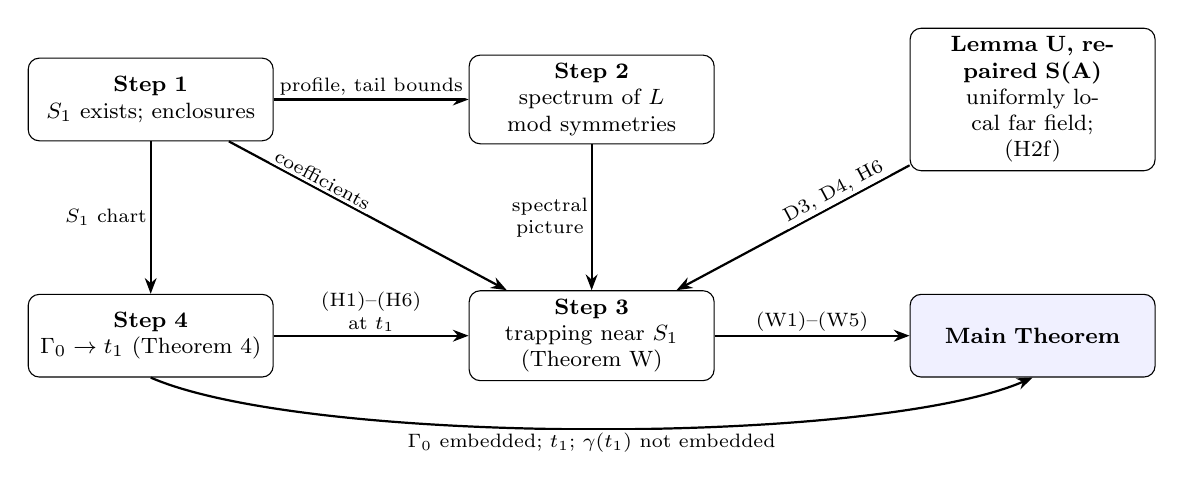
\begin{tikzpicture}[
  box/.style={draw,rounded corners,align=center,font=\footnotesize,minimum height=1.05cm,text width=2.9cm,inner sep=3pt},
  hyp/.style={box,dashed,fill=yellow!12},
  arr/.style={-{Stealth[length=2mm]},thick},
  lab/.style={font=\scriptsize,align=center,fill=white,inner sep=1pt}]
\node[box] (s1) at (0,3) {\textbf{Step 1}\\ $S_1$ exists; enclosures};
\node[box] (s2) at (5.6,3) {\textbf{Step 2}\\ spectrum of $L$ mod symmetries};
\node[box] (F) at (11.2,3) {\textbf{Lemma U, repaired S(A)}\\ uniformly local far field;\\ (H2f)};
\node[box] (s4) at (0,0) {\textbf{Step 4}\\ $\Gamma_0\to t_1$ (Theorem 4)};
\node[box] (s3) at (5.6,0) {\textbf{Step 3}\\ trapping near $S_1$ (Theorem W)};
\node[box,fill=blue!6] (mt) at (11.2,0) {\textbf{Main Theorem}};
\draw[arr] (s1) -- node[lab,above]{profile, tail bounds} (s2);
\draw[arr] (s1) -- node[lab,left]{$S_1$ chart} (s4);
\draw[arr] (s1) -- node[lab,pos=0.32,sloped,above]{coefficients} (s3);
\draw[arr] (s2) -- node[lab,pos=0.5,left]{spectral\\picture} (s3);
\draw[arr] (F) -- node[lab,pos=0.3,sloped,above]{D3, D4, H6} (s3);
\draw[arr] (s4) -- node[lab,above]{(H1)--(H6)\\at $t_1$} (s3);
\draw[arr] (s3) -- node[lab,above]{(W1)--(W5)} (mt);
\draw[arr] (s4.south) .. controls (2,-1.4) and (9.2,-1.4) .. node[lab,below]{$\Gamma_0$ embedded; $t_1$; $\gamma(t_1)$ not embedded} (mt.south);
\end{tikzpicture}
\caption{Dependencies (v3.3). Earlier drafts had the dashed box \emph{Hypotheses (F1), (O)} in place of Lemma~U and the repaired Lemma~S(A); see Remark~\ref{rem:hist}.}\label{fig:dep}
\end{figure}

\section{Step 1: existence of \texorpdfstring{$S_1$}{S1} with tight enclosures}\label{s:step1}
\emph{Documents:} \dref{S1} (Theorem~\ref{thm:S1}), \dref{S1t} (Proposition~2$'$) and the READMEs of \fn{s1_tight}, \fn{ext813}, \fn{ext_tip} and \fn{consistency}.

\emph{Conical ends.} Writing $k'''+\frac\sigma4k=N:=-k(kk'+J)$, $J=\int_\sigma^\infty k'^2$, and diagonalising, a Lyapunov--Perron argument with explicit constants constructs, for every $|\eps|\le1.62\cdot10^{-4}$, a solution of \eqref{eq:prof} on $[8,\infty)$ with a conical end, normalised by $q-\sigma\to0$; the inequalities are checked in Arb at 256 bits. The sharp version replaces the first-order end state by the exact decaying solution $K_j(\sigma)=\frac1{2\pi i}\int_Ct^je^{\sigma t+t^4}dt$ of the linearised end equation, evaluated by validated quadrature with a tail bound; only a remainder cubic in $\eps$ is left, $|d|\le4.37\cdot10^{-13}$.

\emph{Shooting.} CAPD integrates the outward-rounded parallelepiped of end states back to the symmetry line and encloses $M(\eps)$ through a Poincar\'e map:
\begin{gather*}M(1.45\cdot10^{-4})\in[0.04339455686,\,0.04339455704],\\ M(1.62\cdot10^{-4})\in[-0.03933409755,\,-0.03933409733].\end{gather*}
Bisection on certified signs gives the bracket of Table~\ref{tab:S1}.

\emph{Geometry and exports.} Validated checks give the double point, the embedding of each half-branch, the mirror symmetry and the tail. The profile is exported as described in \S\ref{s:data}; conditioning on $M=0$ is valid for every zero of $M$ in $Y$, so no uniqueness is used.

\emph{Trust base.} CAPD's interval ODE solver and Poincar\'e map (FILIB intervals, outward rounding), Arb ball arithmetic and quadrature, and the hand estimates of the tail proposition.

\section{Step 2: linear stability modulo symmetries}\label{s:step2}
\emph{Document:} \dref{S2}.
\begin{theorem}[step 2]\label{thm:step2}
In $L^2(\R,\rho\,dx)$, every eigenvalue of $L$ with $\operatorname{Re}\lambda>-\frac18$ is one of: in the even class $\lambda=1$ $(u=p)$ and $\lambda=\frac14$ $(u=\ip{a_\parallel}\nu)$; in the odd class $\lambda=\frac14$ $(u=\ip{a_\perp}\nu)$ and $\lambda=0$ $(u=q)$. Each is a simple zero of the Evans function of its class. Every eigenvalue with $\operatorname{Re}\lambda\ge-\frac18$ satisfies $\operatorname{Re}\lambda\le1.7909$ and $|\operatorname{Im}\lambda|\le(1.7683-\cos(0.48)\operatorname{Re}\lambda)/\sin(0.48)$.
\end{theorem}
\emph{Method.} (i) Two numerical-range certificates of Legendre--Riccati (sum-of-squares) type, found by a semidefinite program (not trusted) and verified in Arb on the whole line, $\Lambda_0=1.790819$ at $\theta=0$ and $\Lambda_1=1.768282$ at $\theta=0.48$, confine the eigenvalues with $\operatorname{Re}\lambda\ge-\frac18$ to a trapezoid inside the contour $\mathcal C$ with vertices $1.85\pm0.3i$, $-0.125\pm4.1i$. (ii) A Lyapunov--Perron construction at $\sigma_0=32$ gives the admissible plane at the conical end with explicit constants ($202$ boxes along $\mathcal C$, $\eta\le0.1163$, contraction $\le0.272$). (iii) CAPD encloses both Evans functions on $5{,}058$ segments of the upper half of $\mathcal C$; argument cones certify winding number $2$ in each class, and a cover of the interior by $174$ boxes certifies analyticity.

\emph{Remarks.} Numerically the even spectrum is $1,\frac14,-0.2561532,-0.6998896,\dots$, all real; the certified gap is $\frac18$. Only the even class matters for the flow, which preserves the reflection symmetry. That the order of a zero of the Evans function equals the algebraic multiplicity is quoted from the literature \cite{AlexanderGardnerJones1990,KapitulaPromislow2013,LatushkinSukhtayev2010}; its hypotheses have not been checked in this half-line, weighted setting \dref{S2} Remark (Multiplicity).

\section{Step 3: nonlinear trapping near \texorpdfstring{$S_1$}{S1}}\label{s:step3}
\emph{Documents:} v3.1 \dref{S3}; the amendment v3.2, approved by the authors, \dref{S3a}, \dref{S3'}, with Lemma~O v3.2 and Lemma~R \dref{LO}, \dref{LR}; Lemma~S \dref{LS}; the gap note \dref{GAP}. \textbf{v3.3 (this draft):} Lemma~U, the uniformly local far-field estimate \dref{LU}, with the repaired Lemma~S(A) and the new statements \dref{ST}; the file map is \dref{IDX} and the v3.1 erratum is \dref{ERR}.

\begin{theorem}[Theorem W, v3.1 as amended by v3.2 and v3.3; trapping with a floor]\label{thm:W}
Let $\gamma$ be a smooth closed immersed curve moving by CDF, and $t_1$ a time at which:
\begin{enumerate}[label=\textup{(H\arabic*)},leftmargin=*,itemsep=1pt]
\item the modulated decomposition exists, $|\alpha(\tau_1)|\le\alpha_1=1.5\cdot10^{-4}$ and $\sqrt{\Lam(\tau_1)}\le5\cdot10^{-8}$;
\item the shell energies on $y\in[14,60]$ satisfy $E_0\le10^{-8}$, $E_1\le10^{-6}$, $E_2\le10^{-3}$ (tightened from $2\cdot10^{-7},10^{-4},0.2$ of v3.2), and \textup{(H2f)}: $G_j=\int_{60}^{700}\frac{28}y\,z_j^2\,\frac{dy}y\le(10^{-6},5\cdot10^{-6},10^{-5})$ for $j=0,1,2$, with $z_j=(y\partial_y)^j(f-U_1)$;
\item on every window $[y,1.5y]$, $y\in[50,253]$, the deviation energies satisfy $E_0\le2\cdot10^{-7}$, $E_1,E_2,E_3\le10^{-5}$, and the fourth jet satisfies $K_4\le0.06$ on $y\in[50,350]$;
\item the curve is a graph over the $S_1$ ray on $y\in[48,700]$ (v3.2: $[48,350]$; with the verifier's decomposition on $y\le57.75$ this gives the graph property on $[14,700]$ needed by v3.3);
\item the Lemma~O data hold arc by arc for the fixed-$L$ cone family ($L=50\lambda_1$, centres $r\in[300,380]\lambda_1$, $M=0.12$) and the far family (unit $113\lambda_1$, $M=0.15$, centres $\ge490\lambda_1$), with the six data thresholds of v3.2;
\item $\gamma(t_1)$ is smooth, closed and immersed.
\end{enumerate}
The bootstrap closes (by Lemma~U and the repaired Lemma~S(A), \S\ref{ss:gap}; unconditional subject to the pending review), so the solution exists for all $\tau\ge\tau_1$, i.e.\ on $[t_1,T)$ with $T<\infty$, and: \textup{(W1)} $|\alpha|\le1.5\cdot10^{-4}$, $\sqrt\Lam\le5.31\cdot10^{-8}$, with decay to the floor of (iv) of the Main Theorem, and $\sup|a|,\sup|b|\le2.192\cdot10^{-7}$, $\sup|\beta|\le3.34\cdot10^{-9}$; \textup{(W2)} pointwise tip control, e.g.\ $|w'|\le1.161\cdot10^{-3}$, $|w''|\le1.55\cdot10^{-2}$ on $x\ge16.25$; \textup{(W3)} bounds on the shell and uniformly local energies (v3.3 \textup{[cert]}): $E^A_j\le\hat E_j$ with $\hat E=(1.2018\cdot10^{-6},1.0441\cdot10^{-4},0.056694)$ on the shells, core $\sup|v_A|\le7.1878\cdot10^{-3}$, and $\mathfrak E^\rho_j\le\hat B_j$ with $\hat B=(4.8735\cdot10^{-6},5.5933\cdot10^{-4},0.36675)$ for the uniformly local energies at every launched centre $\rho\le253\lambda_1$ (the v3.1 values $E_j\le(3.12\cdot10^{-7},1.81\cdot10^{-4},0.248)$ and $|f|\le0.093$ omitted the edge terms, \S\ref{ss:gap}); \textup{(W4)} on $\{y\ge56,\ r<253\lambda_1\}$: $|f|\le0.15$, $|yf_y|\le0.52$, $|f-U_1|\le0.16$; on $[253,379.5]\lambda_1$: $|f|\le0.10032$, $|rf_r|\le0.41974$; on $r\ge251.44\lambda_1$ the curve is a graph over the Lemma~O cylinders with a-priori bounds $K_2=K_3=0.18$ (cone) and $0.3$ (far), arc by arc; in particular $|f|\le0.15$ on $\{28\le y,\ r<379.5\lambda_1\}$ and the curvature is at most $C/r$ there (this replaces v3.2's ``$|f|\le\frac12$ on $y\in[48,R(\tau)]$ and curvature $\le S_1^f/r$''; $R(\tau)$ and $S_1^f$ are not used in v3.3; \fn{lemmaU_v34.tex}, \fn{continuation_v33.tex}, conclusions (W1)--(W5)); \textup{(W5)} $\lambda\to0$, $T-t_1\le\lambda_1^4/(1-4\bar a)$, $\lambda(t)=(T-t)^{1/4}(1+O(\bar a))$, a single singular point, smooth convergence away from it.
\end{theorem}

\subsection{Components}
All of the following are certified (\dref{S3'} \S3, status tag C) unless stated otherwise.
\begin{itemize}[leftmargin=*,itemsep=1pt]
\item \emph{Linear coercivity.} $\operatorname{Re}\ip{Lv}v_\rho\le-\frac3{64}\norm{v}_\rho^2$ for even $v$ satisfying the three constraints; the modulated semigroup satisfies $\norm{e^{\tau\mathcal L}u}_\rho\le14.8\,e^{-0.0213\tau}\norm u_\rho$.
\item \emph{Forcing, modulation and verifier.} The forcing norms, the modulation bounds (by integration by parts, checked on all hull boxes), and an interval branch-and-bound comparison system for $(\alpha,\Lam)$ with outward rounding throughout. At the hand-off point: peak $\sqrt\Lam\le5.308\cdot10^{-8}$, tail rate $\ge2.693\cdot10^{-3}$, floor $\sqrt{\Lam_F}\le9.872\cdot10^{-10}$ (verifier \fn{fin12f4}), and time integrals $J_{0,1,2}\le(6.03,8.47,1.88)\cdot10^{-12}$, $J_4\le6.24\cdot10^{-8}$.
\item \emph{Lemma S(A) (shells; repaired, v3.3).} Divergence-form energy identities (checked symbolically). The v3.1 proof omitted ramp terms and the outer cutoff on $[350,700]$; the repaired version (\dref{LU} sources \fn{fix2/n12/t2_A_v35}, erratum \dref{ERR}) keeps them, runs on the v3.3 verifier (tag \fn{fin12f4}, flux floors $\times4$), takes as datum the tightened (H2) together with (H2f), and uses $\beta_A=2$ in bootstrap item B2$'$. Certified (final, \fn{t2\_A\_v35}, interface \fn{78fe2f8e...}; margins at $4\times N_2^{\rm ref}$, which dominates the certified $\bar N^2$): $\hat E^A_2\le0.056694$; core $M_1$ margin $\times4.409$; $S_0^v+\sup_{\rm core}|d|$ margin $\times2.116$ (B2$'$: $\sup|v_A|+\sup_{\rm core}|d|\le0.0153$); $G_{22}$ margin $\times1.917$; flux margins $\times3.365$ and $\times5.955$ (the thinnest, at $\beta_A=2$) \textup{[cert]}. The profile difference $d=(f-U)-w'$ is certified in step~4 (stage \fn{b0\_dprof}), and so is the chart term between the verifier's $S_1$-chart variable and the ray graph (stage \fn{n1\_chart}, review N1; it moves every margin by at most $0.06\%$).
\item \emph{Lemma U (uniformly local far-field energies, v3.3; replaces Lemma S(B)).} Energies $\mathfrak E^\rho_j$, $j=0,1,2$, are centred at every physical radius $\rho$, with a weight that never vanishes and one frozen profile $U_1$ for all centres; the transport identity (Lemma~T) keeps the edge and ramp terms that v3.1/v3.2 dropped, and the window form of Lemma~D bounds the data term. Proposition~U gives $\mathfrak E^\rho_j\le\hat B_j$ at every launched centre, by a comparison argument closed in the bootstrap (Proposition~\textup{closure}, with the open--closed argument written out). Certified margins: late centres, core $M_1$ $\times2.353$ and $M_0$ $\times4.892$; present centres $M_1$ $\times2.770$ and $M_0$ $\times2.225$; loop gain $\le0.03904$; rate $\times28.2$; (K6) datum margin $\times1.189$ \textup{[cert]}. The profile-mismatch constant is $c_{\delta U}\le1.7187\cdot10^{-8}$ and the new bootstrap quantity is $M_{1z}=0.534$ (not equal to $M_1$). Zone III $[253,379.5]\lambda_1$ has box $(b_0,b_1,b_z)\le(0.10032,0.41974,0.014291)$ (thinnest margin $\times1.238$ on $b_1$) and outer-ramp error $\Delta^R_2=0.01148$ \textup{[cert]}. Proof text: \dref{LU} (\fn{fix1/lemmaU_rev/lemmaU_v34.tex}, revision v34 of \fn{lemmaU.tex}, numbers and hashes of v35; not compiled); certificates in \fn{t4_cert}, \fn{t5_zone3}. Open points for the review: items G5--G7 of its report.
\item \emph{Lemma O and Lemma R.} Lemma~O is a graph-persistence lemma for the fourth-order flow on cylinders of unit $L$ up to a time ratio $t^*$: certified $t^*\ge3.683\cdot10^{-7}$ against the needed $1.6001\cdot10^{-7}$ (cone, now the fixed-$L$ family with $L=50\lambda_1$; $\times2.30$) and $9.511\cdot10^{-8}$ against $6.134\cdot10^{-9}$ (far; $\times15.5$). Lemma~R (v3.2, certified) bounds the time-averaged $\int h_{xxxx}^2$ on cylinder conclusion regions; in v3.3 the outer cutoff ramp of the energies is $[253,379.5]\lambda_1$ (ramp error $\Delta^R_2=0.01148$ \textup{[cert]}), reached by the fixed-$L$ family.
\item \emph{Theorem H6 (v3.2).} The a-priori bounds of Lemma~O are recovered at every centre, given the strip statement at levels $0$--$2$, which in v3.3 is Lemma~U with the U-fine energies $\hat B^{\rm fine}=(4.8723\cdot10^{-6},2.6266\cdot10^{-4},0.025842)$ \textup{[cert]}: smallest factor $\times1.86$ (far $K_3$), cone slope $\times2.46$, cone $K_2$ $\times2.54$, cone $K_3$ $\times2.51$, $t^*$ $\times2.30$ \textup{[cert]} (v3.2: smallest $1.69$, conditional on (F1) and (O)). Under v3.1 alone H6 is not met.
\end{itemize}

\subsection{The bootstrap}\label{ss:boot}
For $\tau'\ge\tau_1$, $\mathrm{BS}(\tau')$ means that on $[\tau_1,\tau']$: \textbf{B1} $|\alpha|$ and $\sqrt\Lam$ stay below the barrier of the verifier (peak $5.31\cdot10^{-8}$); \textbf{B2} on the core $y\in[28,60]$, $\sup|v|\le0.0153$, $M_0\le0.11$, $M_1\le0.52$ and $E_j\le\beta_A\hat E_j$ ($\beta_A=2$ in v3.3, B2$'$); \textbf{B3} on the far field: in v3.2, $|f|\le\frac12$ on the window region $y\in[48,R(\tau)]$ (here $R(\tau)$ is the outer end of v3.2's window family, step~3 v3.2 \S3.7; it is not used in v3.3), window energies $\le2\times$ their entry values and the per-window boxes; in v3.3 this is B3U: the uniformly local energies satisfy $\mathfrak E^\rho_j\le\hat B_j$ at every launched centre $\rho\le253\lambda_1$ and $|f|\le0.15$, $|yf_y|\le0.52$ on $\{y\ge56,\ r<253\lambda_1\}$ (Lemma~U, \S\ref{ss:gap}); \textbf{B4} the Lemma~O a-priori bounds at all centres (far centres $\ge490\lambda_1$ in v3.3). The steps D1 (verifier), D2 (ramp values), D3 (shells), D4 (windows), D5a/D5b (Lemma~O, Theorem~H6) and D6 (barrier) derive each bound strictly better from $\mathrm{BS}(\tau')$, the hand-off data and the certified constants; a continuity argument and the continuation criterion (P1) then give $\mathrm{BS}$ for all $\tau\ge\tau_1$ \dref{S3'} \S4.

\subsection{The far-field estimate: Lemma U, and the former Hypotheses (F1) and (O)}\label{ss:gap}
\emph{Status in v3.3.} The two hypotheses of earlier drafts are replaced by proofs (Remark~\ref{rem:hist}). \textbf{Lemma~U} (above, \dref{LU}) supplies the far-field energy estimate with the edge terms kept; the \textbf{repaired Lemma~S(A)} (erratum \dref{ERR}) supplies the shell estimate including the outer cutoff on $[350,700]$; and Lemma~N of \dref{LU} derives, inside the bootstrap, the pointwise bounds (H-O1) ($|f|\le\frac12$, $|yf_y|\le1$ on the outer annulus $[350,700]$) and the $L^2$ form (H-O2$'$) of the outer data of Lemma~S(A), $\sup_\tau\int_O(z^A_k)^2ds\le\bar N^2_k$; it does not derive the pointwise (O3) ($|z_k|\le1$ for $k\le3$), which v3.3 does not use. New hand-off items: \textbf{(H2f)} on $[60,700]$ and the tightened (H2), certified in step~4 (arb rows of review M9) with margins $\times3.188,\times4.983,\times4.106$ for (H2f), $\times124.7$ or more for the tightened (H2) of $w'$, and $\times27.34,\times562.8,\times600.9$ for the tightened (H2) in the variable $f-U_1$ \textup{[cert]} (\S\ref{s:step4}). The tightened (H2) is met by step~4's shell energies, about $3\cdot10^{-10}$, with room. \emph{Not yet done:} independent review (task 8), compilation, and the v3.3 reproduction kits; the points G5--G7 of \dref{LU} and the arc-end question of \S\ref{s:step4} are for that review. The remainder of this subsection records the situation of v3.1 and v3.2: earlier drafts of this document were conditional on Hypotheses (F1) and (O), and the present tense in the following paragraphs refers to those versions.

\begin{remark}[Historical: the gap of v3.1 and v3.2]
\emph{Status of Lemma~S(A) (13 November).} An independent review found that the proof of Lemma~S(A) in v3.1 is incomplete: it omits ramp terms (the top pair on the ramp, the cutoff $\times$ jet terms, the profile jets $U_j$ in the coefficients and the flux constant $I_3$). The statement is repaired and holds with corrected constants (erratum \dref{ERR}; certified). At the v3.1 thresholds (erratum \dref{ERR}, column ``repaired, v3.1 setting'', \textup{[cert]}) the repaired energy bound is $\hat E_2\le0.25558$, the core $M_1$ margin is $\times2.723$, the thinnest margins are the flux margin $\times1.146$ at $\beta=2$ ($\times1.124$ with the outer data of (O3)) and the ramp $M_1$ margin $\times1.185$; all repaired margins exceed $\times1$, so no inequality fails. (An earlier draft of this sentence quoted $E_2=0.2686$, $\times2.73$, $\times4.9$, $\times5.3$ and ``all margins at least $\times2$''; these do not match the erratum table and are withdrawn [TODO: source for 0.2686, $\times4.9$, $\times5.3$ if they are to be restored].) The repair does not cover the outer cutoff of Lemma~S(A) on the rescaled interval $[350,700]$, which v3.1 never treated; this is Hypothesis~(O). Hypothesis~(F) was then unchanged as a text, but its part (F2), which postulates the conclusion of Lemma~S(A), was a consequence of the repaired Lemma~S(A) under (O).


Step~3 controls the far field $y\ge60$ by energies on windows fixed in physical space. The energy identities of Lemma~S hold only up to total derivatives \dref{LS} (Prop.~1). On a window the discarded total derivatives are exactly the fourth-order edge terms; with a cutoff, they become ramp commutators. The certified (B) bounds keep entry value times growth, plus forcing and coupling, and nothing else. No source estimates the edge terms or dismisses them: not the step-3 text, not the scripts or their Arb rigor pass, and not the verifier, which never touches the windows. The edges move with the physical scale, but this cancels only the transport flux, not the diffusive fourth-order flux, and the edge terms have no sign. The outer end of the shell energies of Lemma~S(A) is likewise unquantified: their support extends beyond the core $y\le60$, where the coefficients come from the window box $|V|\le\frac12$ and no cutoff term is computed. An independent referee check \dref{REF} confirms all of this.

\emph{What an edge needs.} Bounding an edge at level $j$ needs data for $z_k=(y\partial_y)^kv$ on the cutoff ramp at all later times. With the Cauchy--Schwarz commutator tables certified in v3.2 this means $k\le j+1$. Young's inequality against the window's own dissipation reduces the linear commutators to $k\le j$, but at level~2 the quasilinear foot term still needs $z_3$-type data, and level~1 then needs $z_2$, which rests on level~2. v3.2 supplies such data at the outer edge, inside the Lemma~O region (Lemma~R). It is \emph{unproved at every edge lying in $60\lambda(\tau)\lesssim r<150\lambda_1$, at levels 1 and 2} \dref{GAP} \S1, \dref{REF} \S\S1--2.

\emph{What depends on it.} The trapping argument does. The verifier's inputs ($S_0^v$, $S_1^v$ and the flux constants) come from Lemma~S(A) through D3, and D3 uses B3 in the form $|V|\le\frac12$ beyond $y=60$. The continuity argument must re-derive B3 strictly, and that is D4, the edge-free computation. The continuation step (P1) uses (B) and Lemma~O to control the curvature far out. The conclusions W3 and W4 rest on (B). The hand-off-level strip bounds are affected too, and through them H6 (D4, D5b). The trapping estimates near the tip do not use H6 as such, but only because of v3.2's restructuring (D5a/D5b, Lemma~R): in v3.1, D4 took B4 on $[150,175]$ and D5 took D4 on the strip. \emph{Not affected:} the verifier given its inputs; the core and inner-ramp computations of Lemma~S(A) given a crude far-field box and an outer-cutoff bound; Lemmas~O and~R as local lemmas. Hypothesis~(F1) asks exactly for D3 and D4 with the edge terms kept; in v3.2, under (F1) and (O), the bootstrap would close as written, with the corrected Lemma~S(A) constants.

\emph{Character, and numerical room (evidence, not proof).} The gap is a missing estimate, not a failed inequality. Without the edge terms, the derived $|f|\le0.093$ is a factor $5.38$ below $\frac12$, and the core bounds $M_0\le0.0188$, $M_1\le0.1844$ are factors $5.86$ and $2.82$ below their boxes; Theorem~H6 tolerates strip energies up to $30$ times the per-window values (smallest factor then $1.26$). The edge coefficients are small, e.g.\ $c^{\rm in}_{22}=2.43\cdot10^{-4}$ and $c^{\rm in}_{23}=3.36\cdot10^{-5}$ on the inner strip ramp $[50,75]\lambda_1$. But they multiply ramp norms $\bar N_k^2$ (time averages of $\int_{\rm ramp}z_k^2$) for which step~3 has no bound in $r<150\lambda_1$: H6 needs roughly $c^{\rm in}_{22}\bar N_2^2+c^{\rm in}_{23}\bar N_3^2\lesssim2\cdot10^{-4}$, e.g.\ $\bar N_2^2\le0.4$, $\bar N_3^2\le3$, and the available estimates give about $0.7$ and $10^3$ \dref{LR} \S5. Two repairs were examined and neither is complete. Bounding a window's ramp norms by the dissipation of overlapping windows is circular for physically fixed windows, and its floating-point estimate misses the strip requirement by a factor 40--80 \dref{REF} \S2(d). Co-moving power weights close on floating-point estimates with a margin of about $10$, but need the crude far-field box on the whole support of the weight, which they cannot supply themselves \dref{GAP} \S\S3--4.

\emph{Proposed route.} A uniformly local version of Lemma~S(B): general weights $W$ with $|W^{(m)}|\le\Gamma_mW$ in the divergence-form tables (the weight enters them linearly), launched at every scale. It would give first the crude far-field box, and then, with a fixed-unit family of innermost Lemma~O cylinders, the collar bounds for H6 \dref{GAP} \S4. This route is the one carried out in v3.3 as Lemma~U.
\end{remark}

\subsection{Further caveats of step 3}\label{ss:caveats}
\dref{S3'} \S6 also lists: the frozen-profile reruns take $\cos\theta$ constant along the ray, and the commutator tables behind the ramp coefficients use IEEE-double coefficient bounds; three final-rigor items of Lemma~S (assembly arithmetic in IEEE double, class weights in floating point, a sliver where a cutoff is below $1$), which the Lemma~S rigor pass of 10 November reports closed (assembly and weights redone in Arb and exact rationals, an unconditional sliver bound; \fn{lemmaS/rigor/RIGOR_PASS.md}) but which the step-3 text still lists; the literature facts (P1); and the frame conventions. Convergence to $S_1$ (``upgrade C'') is not claimed.

\section{Step 4: validated integration from \texorpdfstring{$\Gamma_0$}{Gamma0} to \texorpdfstring{$t_1$}{t1}}\label{s:step4}
\emph{Documents:} \dref{S4} (version 2, 39 pp.), \dref{R4}; for v3.3 the addendum \dref{R4v33} (new stages in \fn{step4/p2/v33}, manifest \fn{FINAL_manifest_v33.json}). The step-4 document itself is closed and unchanged.

\begin{theorem}[Theorem 4; \dref{S4} \S1.3]\label{thm:4}
Let $S_1\in\Sset$ and let $\gamma$ be the CDF evolution of $\Gamma_0$. Then: (a) $\Gamma_0$ is smooth, embedded and symmetric about the $x$-axis; (b) $\gamma$ exists and is smooth and symmetric on $[0,t_1]$, where $t_1\in[4.5978574775,4.5978586144]$ corresponds to a good time in base slab~180, and the base curve's maximal curvature at $t_1$ lies in $[2.279\cdot10^4,2.376\cdot10^4]$; (c) there are $\lambda_1>0$ and $c_1$ such that $(\gamma(t_1)-c_1e_1)/\lambda_1$ satisfies (H1)--(H6) of Theorem~\ref{thm:W} (Table~\ref{tab:handoff}), uniformly for every good time in the slab.
\end{theorem}

\emph{The chain.}
\begin{itemize}[leftmargin=*,itemsep=1pt]
\item \emph{P1: validated Fourier slabs.} In Fourier variables for the tangent angle, the flow is integrated through 96 slabs with Chebyshev--Lobatto bases, Lohner-type error blocks and componentwise Duhamel bounds with an $n^{-6}$ tail; a first-exit Galerkin-limit lemma makes this an existence and uniqueness theorem. At slab 96: $t_{96}=4.597850539485830831\pm7.8\cdot10^{-19}$, $k_{\max}\in[29.352874545325,29.352874545328]$, $2800$ modes, $6.24$~h of one core.
\item \emph{Switch and P2.} The P1 enclosure is converted into the modulated chart of a polished piecewise-polynomial base solution in rescaled variables (181 slabs, $\tau\in[0,27.15]$, $k$ from $26.25$ to $2.37\cdot10^4$): $Y(\tau_a)\le6.21\cdot10^{-13}$ against the majorant $\bar Y=10^{-12}$. P2 shadows the base with $\sqrt{\Lam_e}\le\bar Y$, using the base residuals computed directly on the corrected base, 26 coercivity certificates ($\min c_I\ge0.05284$), a certified nonlinear closure ($\min\varrho_c\ge0.04711$), a certified tip box and far-field lemmas.
\item \emph{Hand-off.} The step-3 coordinates are computed by a Krawczyk/implicit-function test at 16 exact points and 32 derivative balls covering base slab~180 ($k\in[2.27,2.38]\cdot10^4$), and every hand-off item is certified uniformly on the slab.
\item \emph{v3.3 stages (new, \dref{R4v33}).} Twenty further stages, run by \fn{final_tail_v33.py}, certify the items that step~3 v3.3 needs beyond v3.2. Ten stages: (H2f) on $[60,700]$ (widened parameter balls, base sums on $x\in[45,725]$, error-transfer constants, the (H2f) assembly), the tightened (H2) (re-assembly of pinned outputs), and for the fixed-$L$ cone cylinders the jets and (H5) data, Lemma~O~H4, the Lemma~O~H1 graph test and the time ratio H7, and the covering notes. Two B0 stages: the profile difference $d$ (\fn{b0\_dprof}) and the tightened (H2) in the variable $f-U_1$ (\fn{h2u\_v33}). One N1 stage (re-review N1): \fn{n1\_chart}, the certified bounds on the chart term between the verifier's $S_1$-chart variable and the ray-graph variable on the ramp $[14,28]$ and the core (it replaces a typed level-0 allowance $2\cdot10^{-7}$ of the datum code, which only widened enclosures and is harmless). Every stage now runs with an explicitly constructed environment that the manifest records (re-review N2). Seven M9 stages (review M9): arb window, shell and (H2f) base sums over all 32 parameter balls and both ball sets, the (H3), (H2), tightened (H2), (H2) for $f-U_1$ and (H2f) assemblies on those arb bases, the Lemma~O~H1 check with a certified centre map, and the far-family Lemma~O~H4 at every centre of hand-off radius $\ge490$ (minimum margin $\times15.58$). The arb rows supersede the float rows; no margin moves by more than $7.5\cdot10^{-5}$ (relative). The manifest \fn{p2/out_v33/FINAL_manifest_v33.json} (sha256 \fn{a0d348ec2dfb84bd3c62482517a0aa26f5d29ab3e4230081384054f395f8e357}) pins 20 stages, 289 paths and 37 scripts, reuses 85 pinned v3.2 files (checked against \fn{FINAL_manifest.json}, which stays unchanged: 34 stages, 523 paths), and is written atomically and resumably. All passes \textup{[cert]}.
\end{itemize}

\begin{table}[htbp]\centering\small
\caption{Hand-off items at $t_1$ (selection; \dref{S4} Tables 1, 2; \dref{R4} \S\S2, 6, with the values after the final clean-up). A margin is threshold over bound; ``in $\bar Y$'' means the item holds for $\bar Y$ up to that factor times $10^{-12}$.}\label{tab:handoff}
\footnotesize
\begin{tabular}{@{}p{0.22\linewidth}p{0.19\linewidth}p{0.41\linewidth}r@{}}\toprule
item & required & certified & margin\\\midrule
(H1) $|\alpha|$ & $1.5\cdot10^{-4}$ & $1.1739\cdot10^{-4}+7.3\cdot10^{-13}$ & $\times1.27$\\
(H1) $\sqrt\Lam$ & $5\cdot10^{-8}$ & $2.29\cdot10^{-8}$ & $\times2.18$\\
(H2) shells, tightened (v3.3) & $(10^{-8},10^{-6},10^{-3})$ & base $(8.02\cdot10^{-11},1.34\cdot10^{-10},2.94\cdot10^{-10})$ & $\times124.7$ ($j=0$); $\times2124$, $\times641$ with error\\
(H2) tightened, variable $f-U_1$ (v3.3, \fn{h2u\_v33\_arb}) & $(10^{-8},10^{-6},10^{-3})$ & $(3.658\cdot10^{-10},1.777\cdot10^{-9},1.665\cdot10^{-6})$ & $\times27.34$, $\times562.8$, $\times600.9$\\
(H2f) $[60,700]$ (v3.3) & $(10^{-6},5\cdot10^{-6},10^{-5})$ & base $(3.127\cdot10^{-7},1.004\cdot10^{-6},2.431\cdot10^{-6})$; with error $(3.137\cdot10^{-7},1.0034\cdot10^{-6},2.436\cdot10^{-6})$ & $\times3.188$, $\times4.983$, $\times4.106$\\
(H3) windows & $2\cdot10^{-7}$; $10^{-5}$ & base $(3.48\cdot10^{-8},1.27\cdot10^{-7},3.76\cdot10^{-7},9.71\cdot10^{-7})$ & $\times15.7$ in $\bar Y$\\
(H3) $K_4$ & $0.06$ & $5.60\cdot10^{-3}$ & $\times10.7$\\
(H4) graph & over the ray & $|\theta-\Theta|\le0.078+5.5\cdot10^{-4}$ & ---\\
(H5) fixed-$L$ cone slope datum (v3.3) & $0.08$ & $0.03029$ & $\times2.64$\\
(H5) fixed-$L$ cone $\sup|h_0''|$ datum (v3.3) & $0.03$ & $0.009876$ & $\times3.03$\\
(H5) Lemma O H4 & $\int(h_0^{(5)})^2\le M^2$ & $1.2865\cdot10^{-5}$ (fixed-$L$ cone, threshold $0.0144$); $0.1761\,M^2$ (far) & $\times1119$; $\times5.68$\\
(H5) far-family Lemma O H4, every centre at radius $\ge490$ (v3.3, \fn{h4far\_v33}) & $\int(h_0^{(5)})^2\le M^2=0.0225$ & $1.444\cdot10^{-3}$ $(0.0642\,M^2)$ at the worst row (centres $471$--$584$, base arclength) & $\times15.58$\\
(H5) fixed-$L$ cone H7 & $t^*\ge$ ratio & ratio $\le1.6000014\cdot10^{-7}$, $t^*\ge3.68334\cdot10^{-7}$ & $\times2.30$\\\bottomrule
\end{tabular}\end{table}

\emph{Review.} An independent review found three gaps (an unchecked Lemma~O hypothesis H4, nonlinear terms carried only as an allowance, an uncertified tip box) and nine further findings; all are resolved \dref{S4} \S1.6. The thinnest certified margins of step~4 are $|\alpha|$ ($\times1.27$), the cone slope datum of v3.2 ($\times1.40$; $\times2.64$ for the fixed-$L$ family of v3.3), the cone $\sup|h_0''|$ datum of v3.2 ($\times1.59$; $\times3.03$ in v3.3), the initial error $Y(\tau_a)$ against $\bar Y$ ($\times1.6$) and the far $|e|$ box ($\times1.69$; the $|e'|$ box has $\times6.42$) \dref{R4}. The step-4 computation of the v3.2 H6 closure (smallest factor $1.69$) rested on the strip input that was then Hypotheses (F1) and (O); in v3.3 it is superseded by the H6 computation of step~3 (smallest factor $\times1.86$, \S\ref{ss:gap}). One point is for the independent review: the v3.2 script for the cone Lemma~O~H1 did not test $|\xi|>X_L$ at the arc ends; the v33 copy does, on an arc lengthened from $1.1X_L$ to $1.3X_L$, and whether closed v3.2 needs an erratum for this is undecided \dref{R4v33}.

\section{Computer assistance}\label{s:cap}

\subsection{Arithmetic}
\begin{itemize}[leftmargin=*,itemsep=1pt]
\item \emph{Ball arithmetic.} Arb \cite{Johansson2017} through python-flint (midpoint--radius balls, 96--256 bits) for the tail theorems of steps 1--2, the step-2 certificates, Lemmas O and R, the Lemma~S assembly, and all of step~4. The step-3 verifier uses double-precision intervals rounded outward at every operation, with 200-bit Arb constants.
\item \emph{Interval ODE solvers.} CAPD \cite{CAPD2021} (FILIB intervals, outward rounding) for the $S_1$ enclosures, Poincar\'e maps and the Evans functions ($C^0$ and $C^1$ Lohner methods).
\item \emph{Existence tests.} Krawczyk operators \cite{Krawczyk1969} for the closure of $\Gamma_0$ and the hand-off modulation; first-exit (isolation) arguments for P1, in the spirit of \cite{Zgliczynski2004}; argument cones for winding numbers.
\item \emph{Floats find, intervals check.} Floating point is used to find objects: semidefinite certificates, collocation and Lohner bases, the polished base, step sizes. Every certified statement is about the exact data produced (dyadic centres, stored balls), whose residuals are enclosed. No certified bound comes from sampling. Symbolic identities are checked offline (sympy), never used as run-time bounds.
\item \emph{Rounding.} Balls stored as doubles are widened outward (\fn{nextafter}); JSON outputs are read back exactly; typed inputs passed between stages are checked against the outputs they come from. Quoted numbers are rounded outward.
\end{itemize}

\subsection{What is computed}
Step~1: the conical-end constants and Laplace-integral end states (Arb), the shooting and profile enclosures (CAPD), the geometric checks. Step~2: two numerical-range certificates on the whole line, the Lyapunov--Perron constants at $\sigma_0=32$, Evans-function enclosures on $5{,}058$ segments. Step~3: the coercivity certificate, the modulation constants on all hull boxes, the verifier's comparison system, the repaired Lemma~S(A) constants, the Lemma~U certificates and the zone-III box (v3.3), the Lemma~O and Lemma~R constants. Step~4: the $\Gamma_0$ certificate, 96 P1 slabs, the switch, residuals and coercivity certificates of P2, the far-field constants, and the hand-off items, and the v3.3 stages ((H2f), tightened (H2), fixed-$L$ cone cylinders).

\subsection{Manifests and kits}
The final part of step~4 runs as one command that writes a manifest (\fn{step4/p2/out/FINAL_manifest.json}): 34 stages in order, among them the far-family Lemma~O~H1 check and the axis crossing, each with its command, environment and the SHA-256 of its inputs and outputs, plus the hashes of 97 upstream files. A second manifest, \fn{step4/p2/out_v33/FINAL_manifest_v33.json}, pins the 20 v3.3 stages (289 paths, 37 scripts; 85 reused v3.2 files verified against the first manifest), and the first manifest is verified before and after it. Second passes reproduce the outputs byte for byte, apart from timing fields (\dref{S4} App.~A.3, \dref{R4} \S3). Reproduction kits: \fn{kit_step3.zip} (step~3 as of v3.1), \fn{kit_step4a.zip} ($\Gamma_0$ and P1; a revised checker is in \fn{kit_step4a_v3.zip}); kit~B (base, P2 and hand-off) is in preparation. None of the kits yet contains the v3.3 additions (verifier \fn{fin12f4}, repaired Lemma~S(A), Lemma~U certificates, zone III, the v33 stages); the list of what they need is in \fn{KITS_TODO.md}.

\subsection{Independent reproduction}\label{ss:repro}
The authors ran the kits on their own machine (Windows~11, Intel i7-10700).
\begin{itemize}[leftmargin=*,itemsep=1pt]
\item \emph{Step-3 kit:} 91 PASS, 0 FAIL, 0 WARN; the verifier is bit-identical to the reference. The kit predates v3.2 and v3.3: Lemma~R, the H6 closure, the frozen-profile reruns, Lemma~U and the repaired Lemma~S(A) are not in it.
\item \emph{Kit A:} the $\Gamma_0$ certificate is bit-identical (the $b_n$, the 192-bit $b_2$ centre and half-width, the arc nodes; Krawczyk contraction $3.01\cdot10^{-12}$). All 96 P1 slabs validate, without retries, and the final slab-96 enclosures overlap the reference; e.g.\ $k_{\max}\in[29.352874545326006,29.352874545327026]$ against $[29.352874545325992,29.352874545327012]$. Intermediate enclosures need not overlap: platform floating point changes the step sizes, so slab-end times differ (by up to $8.7\cdot10^{-16}$), and from slab 82 on the discrete choices differ too. Transported to a common time, all 97 slab-end enclosures of the length $L$ and of $X_0$ agree (a sanity check outside the proof).
\item \emph{Kit B:} pending.
\end{itemize}

\section{Related work}\label{s:rel}
\emph{Loss of embeddedness and convexity.} Giga and Ito proved that an embedded closed curve moved by CDF can lose embeddedness \cite{GigaIto1998} and that a convex one can lose convexity \cite{GigaIto1999}; Mayer and Simonett proved that surface diffusion can drive embedded hypersurfaces to self-intersections \cite{MayerSimonett2000}, and Blatt proved loss of convexity and embeddedness for a large class of higher-order flows \cite{Blatt2010}. Escher, Mayer and Simonett gave numerical simulations of singularities for immersed curves \cite{EscherMayerSimonett1998}. For the related elastic flow of curves see \cite{DziukKuwertSchatzle2002}.

\emph{Global behaviour and blow-up criteria.} Near circles, CDF exists globally \cite{ElliottGarcke1997} and converges exponentially to a circle \cite{Wheeler2013}; for surfaces near spheres see \cite{EscherMayerSimonett1998,Wheeler2012}, and for curves near multiply covered circles \cite{MiuraOkabe2021}. Chou gave a sharp criterion for finite-time blow-up \cite{Chou2003}, and Escher and Ito sufficient conditions for finite-time singularities of surface diffusion and related flows \cite{EscherIto2005}.

\emph{Self-similar solutions.} Edwards, Gerhardt-Bourke, McCoy, Wheeler and Wheeler classify the stationary solutions of CDF, study shrinkers, translators and rotators, and give an explicit shrinking figure eight \cite{EGMWW2015}. Self-similar solutions with contact-angle boundary conditions are studied in \cite{AsaiGiga2014}, and solitons that are entire graphs are classified in \cite{RybkaWheeler2024}. $S_1$ is a shrinker with conical ends and one transverse double point; it was found numerically in \dref{OW}, and step~1 proves its existence.

\emph{Pinch-off by surface diffusion.} For axisymmetric surfaces, Bernoff, Bertozzi and Witelski studied the dynamics and stability of self-similar pinch-off \cite{BernoffBertozziWitelski1998}. Wheeler \cite{Wheeler2026} constructs surface diffusion flows of tori in $\R^3$ that pinch off in finite time: the flow stays embedded up to the singular time, the singularity is modelled on a rigorously constructed positive, even, conical profile (the construction of the profile is computer-assisted), and the initial tori form an infinite-dimensional $C^1$ family of finite codimension. He describes this as the first rigorous example of finite-time singularity formation for surface diffusion realised by a compact embedded trajectory.

Our work is complementary. It concerns plane curves rather than surfaces in $\R^3$; a single explicit initial curve rather than a family; and a non-embedded singularity model, so that embeddedness is necessarily lost before the singular time, whereas in \cite{Wheeler2026} it is kept up to the singular time. Our proof is computer-assisted in every step, including the dynamics; in \cite{Wheeler2026} the dynamics is analytic (gluing, weighted spectral theory, a Lyapunov--Perron selection). And our result is, at present, unconditional only subject to the pending independent review of the new step-3 text and its compilation (status box). We are not aware of an earlier proof of a finite-time singularity of curve diffusion flow from an embedded closed curve.

\emph{Computer-assisted proofs.} For surveys of computer-assisted proofs in PDE see \cite{GomezSerrano2019}; for validated integration of dissipative and semilinear parabolic PDEs see, e.g., \cite{Zgliczynski2004,vandenBergBredenSheombarsing2024}. Computer-assisted proofs of singularity formation include the work of Chen and Hou on the 2D Boussinesq and 3D Euler equations with boundary \cite{ChenHou2022,ChenHou2023}. The Evans-function method behind step~2 goes back to \cite{AlexanderGardnerJones1990}; see \cite{KapitulaPromislow2013}.

\section{Open items and status}\label{s:open}
\begin{enumerate}[label=\textbf{\arabic*.},leftmargin=*,itemsep=2pt]
\item \textbf{Independent review of the v3.3 step-3 text} (task 8, pending). Lemma~U and the repaired Lemma~S(A) have been written and certified by AI agents under the authors' direction; no independent reader has checked them. Points flagged for it: normalisation of $N_3^2$ in the closure (G5); absence of integrations by parts of $(\eta^2)'''$ and $(\chi^2)'''$ in the outer ramp and global $\hat G$ (G6); design choices (ramp box set to the core box, far centres $\ge490$, $M_{1z}=0.534$ per region; G7) \dref{LU}.
\item \textbf{Compilation.} \fn{lemmaU.tex} and this document have not been compiled (no \LaTeX\ on the working machine); balance of braces and environments was checked by script only.
\item \textbf{Hypothesis status.} Hypotheses (F1) and (O) of earlier drafts are removed (Remark~\ref{rem:hist}). Hand-off items that step~3 v3.3 assumes and step~4 certifies: (H2f), tightened (H2), the fixed-$L$ cone cylinders, $\alpha_1$; (H3) unchanged; (H4) on $y\in[48,700]$. The far-family Lemma~O~H4 coverage caveat of earlier drafts (step~4 certified centres $376$ and $602$ only) is closed by the M9 stage \fn{h4far\_v33} (every centre at radius $\ge490$, minimum margin $\times15.58$). The chart identification of the verifier's variable with the ray graph (re-review N1) is closed by the stage \fn{n1\_chart} and the chart lemma of \fn{lemmaS\_A\_v33.tex}. The verifier's tail lemma (W2) and the literature facts (P1)--(P3) are as before.
\item \textbf{Erratum.} The v3.1 erratum for Lemma~S(A) is in \fn{erratum/erratum.tex}; closed v3.1 files are unchanged.
\item \textbf{Lemma~O~H1 arc ends.} The v3.2 cone H1 script did not test $|\xi|>X_L$ at the arc ends (\S\ref{s:step4}); whether closed v3.2 needs an erratum is to be decided.
\item \textbf{Step-3 caveats} (\S\ref{ss:caveats}): frame conventions, the literature facts (P1), and the items of \dref{S3'} \S6, three of which the Lemma~S rigor pass reports closed.
\item \textbf{Step 4} (\dref{S4} \S11, \dref{R4} \S3): the true curve's maximal curvature at $t_1$ is not certified (only the base value; step~3 does not use it), and minor items of \dref{S4} \S11 remain, none of which changes a conclusion. The step-4 document (version~2) predates the final clean-up of \dref{R4} and the v3.3 stages (\dref{R4v33}).
\item \textbf{Reproduction:} kit~B (P2 and the hand-off) has not been run end to end; none of the kits contains the v3.3 additions (\fn{KITS_TODO.md}). The authors decide whether to build and run them.
\item \textbf{Literature:} (P1) in step~3 is cited as Dziuk--Kuwert--Sch\"atzle \cite{DziukKuwertSchatzle2002} Theorem~3.1 and/or Chou \cite{Chou2003} \textbf{[to be confirmed by the authors]}; precise references for (P2), (P3); the multiplicity statement quoted in step~2.
\end{enumerate}

\section{AI-use statement (draft for the authors to edit)}\label{s:ai}
\noindent\rule{\linewidth}{0.4pt}\par\nobreak\smallskip
{\small\textbf{[Draft.]} The mathematical program, the hair-clip scenario in which an embedded curve develops under CDF a singularity modelled on the one-loop shrinker $S_1$, is the authors'. It is set out in their working notes \dref{OW}; the notes record that their numerical experiments and drafting were done by Claude (Anthropic) at M.~Warren's request.

The computations, the code, the certificates and design notes, and much of the drafting were produced by Anthropic's Claude models acting as agents under the authors' direction. The documents record this: the step-1 and step-2 supplements are signed ``Proof, code and draft by Claude (Anthropic) at M.~Warren's request'', the step-3 documents were assembled by Claude, and the step-4 document was assembled by Claude from the project files. This document was drafted by Claude from the project files at the authors' request; Claude also checked its bibliographic data against publisher, arXiv and database pages. The authors directed the work, made the decisions recorded in the documents (for example, the approval of the step-3 amendment v3.2), and reproduced key computations on their own hardware (\S\ref{ss:repro}).

Independent reviews, each by a separate AI model run, found gaps in steps~3 and~4 (\fn{STEP3_REVIEW.md}, \fn{STEP3_REVIEW2.md}, \fn{STEP4_REVIEW.md}); these were then fixed. For example, the step-4 review found three gaps and nine further findings, all since resolved. A further independent AI-assisted review (13 November) found and repaired omissions in the proof of Lemma~S(A) (ramp terms; erratum \dref{ERR}). The far-field gap, formerly Hypotheses~(F1) and~(O), was identified during the work on the step-3 amendment and is stated in the gap note \dref{GAP}; an independent referee check \dref{REF} confirmed it and corrected details of its statement. On 13 November, at the authors' direction, Claude agents wrote the v3.3 text that removes it (Lemma~U and the repaired Lemma~S(A); the statements, the proof text, the certificates in arb, zone III, the new step-4 stages and this assembly were each produced by a separate agent run). \emph{This v3.3 material has not yet been independently reviewed; that review is pending.} \emph{[Authors: say who carried out the referee check.]}

\emph{[Authors: state which parts you have checked by hand, and add the usual statement of responsibility.]}\par}
\noindent\rule{\linewidth}{0.4pt}

\appendix
\section{Project documents}\label{app:docs}
Paths are relative to \fn{/home/claude/}.
\begin{center}
\footnotesize
\begin{tabular}{@{}lp{0.30\linewidth}p{0.56\linewidth}@{}}\toprule
label & document & path\\\midrule
\dref{OW} & Ogden--Warren working notes (25 Sep 2026) & \pth{cdf_blowup_notes.pdf} (upload)\\
\dref{S1} & step-1 supplement: existence of $S_1$ & \pth{s1_cap/s1_proof.tex}\\
\dref{S1t} & sharper enclosure of $S_1$; profile exports & \pth{s1_tight/s1_tight.tex}; READMEs in \pth{s1_tight/}\\
\dref{S2} & step 2: linear stability & \pth{s1spec/writeup/step2_proof.tex}\\
\dref{S3} & step 3, v3.1 & \pth{s1spec/writeup/step3_proof/step3_proof.tex}\\
\dref{S3a} & amendment v3.2 & \pth{s1spec/writeup/step3_amend_v32/amend_v32.tex}\\
\dref{S3'} & step 3, v3.2 & \pth{s1spec/writeup/step3_proof_v32/step3_proof_v32.tex}\\
\dref{LO}, \dref{LR} & Lemma O v3.2; Lemma R & \pth{s1spec/writeup/lemmaO_v32/lemmaO_v32.tex}, \pth{lemmaR.tex}\\
\dref{LS} & Lemma S & \pth{s1spec/writeup/lemmaS/lemmaS.tex}\\
\dref{GAP} & the far-field localisation gap & \pth{s1spec/writeup/step3_gap_v32/gap_v32.tex}\\
\dref{REF} & referee check of the gap & \pth{s1spec/writeup/step3_gap_v32/REFEREE_check.md}\\
\dref{S4} & step 4, version 2 & \pth{s1spec/writeup/step4_proof/step4_proof.tex}\\
\dref{R4} & step-4 result summary & \pth{s1spec/step4/STEP4_RESULT.md}\\
\dref{LU} & Lemma U (v3.3), proof text and certificates & \pth{s1spec/writeup/lemmaU/bulk/t3_proof/lemmaU.tex}; \pth{t4_cert/}, \pth{t5_zone3/}, \pth{t2_A_v33/}\\
\dref{ST} & v3.3 statements (r2) & \pth{s1spec/writeup/lemmaU/bulk/t1_statements/STATEMENTS_r2.tex}\\
\dref{R4v33} & step-4 addendum for v3.3 & \pth{s1spec/writeup/lemmaU/bulk/t7_assembly/STEP4_RESULT_v33_addendum.md}; \pth{s1spec/step4/p2/v33/T6_REPORT.md}\\
\dref{IDX} & v3.3 file map and rerun sequence & \pth{s1spec/writeup/lemmaU/bulk/t7_assembly/V33_INDEX.md}\\
\dref{ERR} & v3.1 erratum (Lemma S(A)) & \pth{s1spec/writeup/lemmaU/bulk/t7_assembly/erratum/erratum.tex}\\\bottomrule
\end{tabular}\end{center}

\bibliographystyle{amsplain}
\bibliography{main}
\end{document}
